\chapter{AODV}
\label{chap:aodv}

\section{Ejercicio 1.1}

\subsection{¿Qué nodos reenvían el primer paquete RREQ enviado por static1? ¿Y el segundo RREQ? ¿Por qué?}

El primer paquete RREQ enviado por static1 es recibido y reenviado únicamente por los nodos mobile[10] y mobile [12], a pesar de enviarse con intención de alcanzar todos los nodos de la red (Figura \ref{fig:primer_rreq_reception}). Esto ocurre porque el primer envío contiene un TTL igual a 2 (aparece en la documentación de Inet), por lo que solamente van a responder los dispositivos a los que le llegue un TTL > 1 para asi poder hacer el reenvío.

El segundo RREQ es reenviado por 10, 12, 3, 1, 7, 2. Al hacer el segundo reenvío, el TTL del paquete pasa a ser 4 (según la documentación de INET, en los siguientes paquetes, el TTL se suma 2 con respeto al anterior ya que el objetivo es poder llegar lo más lejos posible). Como ahora el TLL es 4, pasa por 10 y 12 otra vez (el TTL pasa a ser 3), 12 no alcanza ningún objetivo pero 10 logra mandar ese paquete a 1 y 3 (el TTL pasa a ser 2) y como 3 llega alcanzar a 7 y 2, se los envía también. Llegados a este punto, el TTL es 1 por lo que ya que se acabaría todos los posibles reenvíos del segundo RREQ.

\begin{figure}[H]
    \centering
    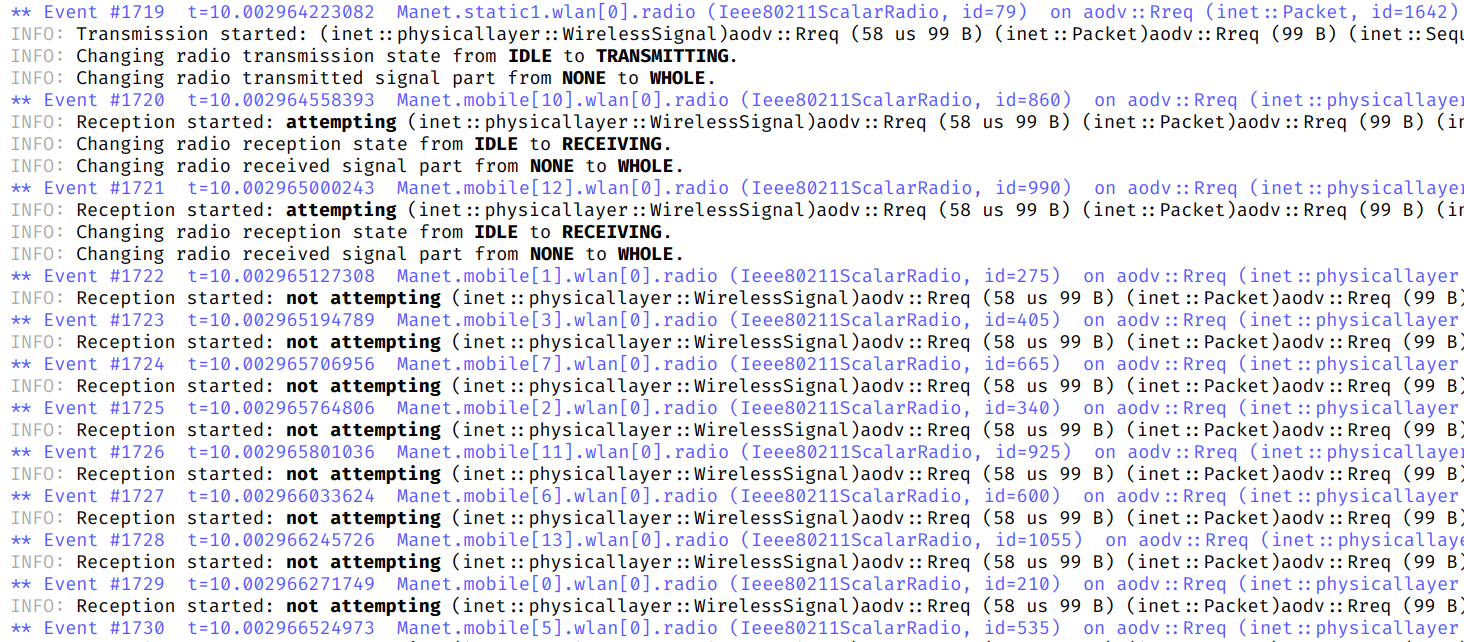
\includegraphics[width=135mm, scale=0.75]{imaxes/ejercicio1_1.png}
    \caption{Logs que muestran el envío del primer RREQ y los nodos que lo reciben}
    \label{fig:primer_rreq_reception}
\end{figure}

\begin{figure}[H]
    \centering
    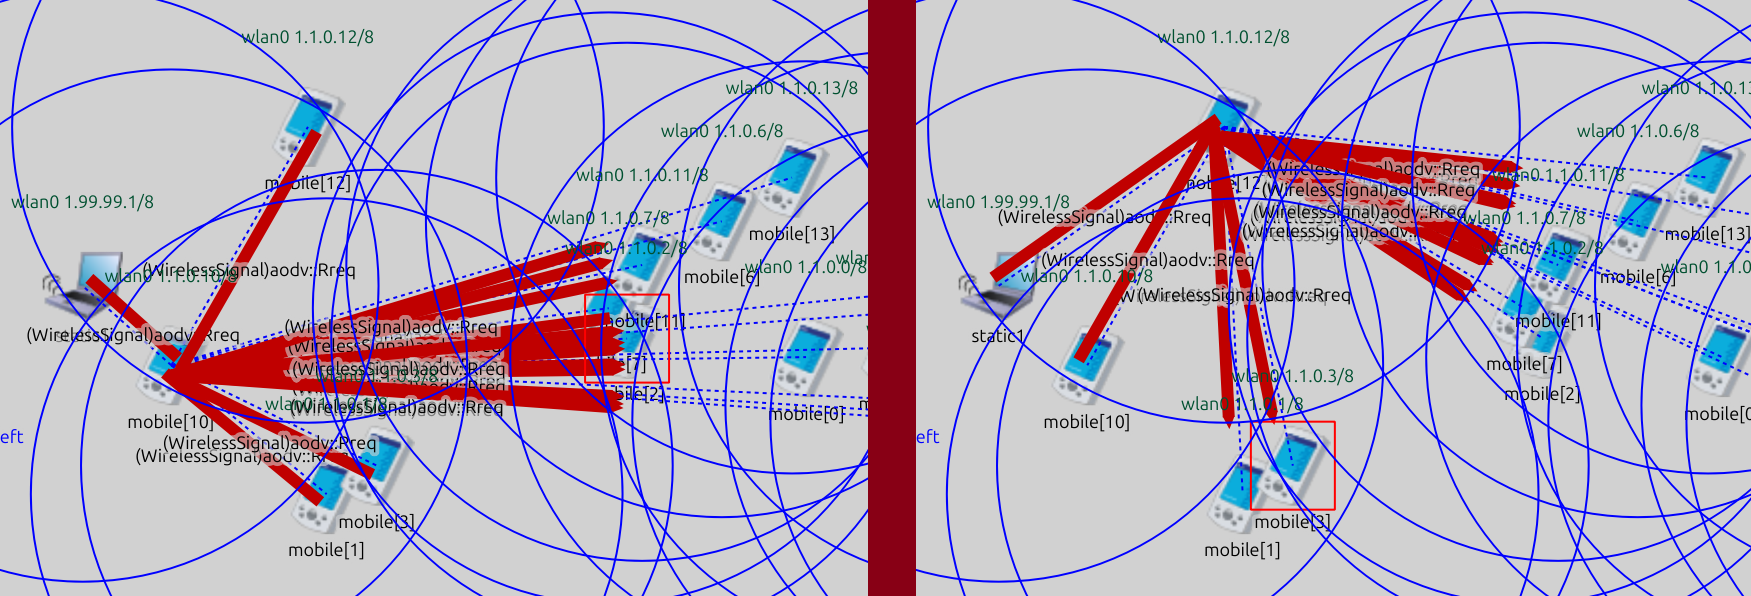
\includegraphics[width=135mm, scale=0.75]{imaxes/ejercicio1_2.png}
    \caption{Nodos que reenvían el primer RREQ (A la izquierda, mobile[10]; A la derecha, mobile[12])}
    \label{fig:primer_rreq_transmission}
\end{figure}


\section{Ejercicio 1.2}

\subsection{Elige el nodo intermedio de la ruta que sigue el primer paquete RREQ que llega a static2. Muestra su tabla
de enrutamiento (vector <Ipv4route *> dentro del módulo ipv4.routingTable) justo antes y justo después de
recibir el primer RREQ. Explica las diferencias y cómo se crean las entradas que aparecen (incluyendo los campos
más importantes).}

\section{Ejercicio 1.3}

\subsection{Haz lo mismo justo antes y justo después del primer RREP.}

\section{Ejercicio 1.4}

\subsection{Tras aplicar la nueva configuración, ¿Cuál es el primer nodo en darse cuenta de la caída? ¿Cómo? Muestra una captura del log del nodo que se da
cuenta que muestre el motivo. ¿Notifica este nodo la caída del nodo?}

\section{Ejercicio 1.5}

\subsection{Muestra el contenido del paquete RERR en Wireshark explicando los campos más importantes. ¿Qué IP
tiene como destino? ¿Por qué?}

\section{Ejercicio 1.6}

\subsection{Explica cómo se propaga el RERR por la red. ¿Qué nodos lo reenvían? ¿Cómo sabe un nodo si debe reenviar
el RERR?}

\section{Ejercicio 1.7} 

\subsection{Muestra capturas de la tabla de enrutamiento de un nodo antes y después de recibir un RERR y explica en
qué cambia.}

\section{Ejercicio 1.8}

\subsection{¿Qué hace static1 al recibir el RERR? Muestra el contenido del siguiente RREQ en Wireshark. ¿En qué cambia
con respecto al de la pregunta 1?}